% Final project report, LaTeX edition. Same layout as the midsem report.
% Numbers, tables and interpretive prose come from generated.tex, which
% report/build_tex.py writes from results/ and report/findings.json.
\documentclass[10pt,twocolumn]{article}
\usepackage[a4paper,margin=18mm,columnsep=6mm]{geometry}
\usepackage{iftex}
\ifXeTeX  % tectonic: TeX Gyre Termes is the Times clone it ships
  \usepackage{fontspec}
  \setmainfont{texgyretermes}[Extension=.otf,UprightFont=*-regular,BoldFont=*-bold,
    ItalicFont=*-italic,BoldItalicFont=*-bolditalic]
\else
  \usepackage{times}
\fi
\usepackage{amsmath,amssymb}
\usepackage{booktabs,tabularx,array}
\newcolumntype{L}{>{\raggedright\arraybackslash}X}
\newcolumntype{P}[1]{>{\raggedright\arraybackslash}p{#1}}
\usepackage{graphicx}
\usepackage{titlesec}
\usepackage{enumitem}
\usepackage[font=small,labelfont=bf,labelsep=colon]{caption}
\usepackage{float}
\usepackage{algorithm}
\usepackage[noend]{algpseudocode}
\usepackage{tikz}
\usetikzlibrary{positioning,arrows.meta}
\usepackage[most]{tcolorbox}
\usepackage{xcolor}
\usepackage{cite}
\usepackage[hidelinks]{hyperref}

\graphicspath{{../../results/figures/}}
\input{generated}

\definecolor{sfred}{HTML}{A8322D}
\newcommand{\SF}{\textcolor{sfred}{\textbf{silent failure}}}
\newcommand{\SFs}{\textcolor{sfred}{\textbf{silent failures}}}
\newcommand{\SFcap}{\textcolor{sfred}{\textbf{Silent failure}}}
\newcommand{\SFscap}{\textcolor{sfred}{\textbf{Silent failures}}}
\newcommand{\phat}{\hat{p}}

\titleformat{\section}{\normalsize\bfseries\scshape}{\thesection.}{0.5em}{}
\titleformat{\subsection}{\normalsize\bfseries}{\thesubsection}{0.6em}{}
\titlespacing*{\section}{0pt}{1.2ex plus .5ex}{0.6ex}
\titlespacing*{\subsection}{0pt}{1ex plus .4ex}{0.4ex}
\setlist{leftmargin=*,itemsep=1pt,topsep=2pt}
\renewcommand{\algorithmicrequire}{\textbf{Input:}}
\renewcommand{\algorithmicensure}{\textbf{Output:}}
\algrenewcommand\algorithmiccomment[1]{\hfill{\color{gray}$\triangleright$ #1}}
\setlength{\textfloatsep}{8pt plus 2pt}
\setlength{\floatsep}{6pt plus 2pt}

\title{\Large\bfseries Catching Silent Failures: Reliability and Failure Topology of Autonomous LLM Agents in
Data Analysis Pipelines}
\author{%
  \begin{tabular}{cc}
    Shaurya Mittal Nair & Pragun Kathuria\\
    Roll No. 2410110316 & Roll No. 2410110237
  \end{tabular}\\[2pt]
  {\small Department of Computer Science and Engineering, Shiv Nadar Institution of Eminence}\\
  {\small Final Project Report, Foundations of Data Science (CSD355)}\\
  {\small \url{https://github.com/Uncharted1804/agent-reliability}}}
\date{October 2026}

\begin{document}
\maketitle

\section*{Abstract}
\FAbstract

\begin{tcolorbox}[enhanced,colback=sfred!6,colframe=sfred,boxrule=0pt,leftrule=2.5pt,arc=0pt,
  left=5pt,right=5pt,top=4pt,bottom=4pt,fontupper=\small]
\textbf{Silent failure: the object of this study.} A \SF{} is an agent run that ends normally and returns
a clean, well-formed, confident answer that is \textbf{wrong}. Nothing raises an exception, nothing is logged as an
error, no retry fires and no warning is shown, so every monitor that watches for crashes reports success. It is the
opposite of a \emph{visible failure} (a crash, an error, an empty or unparseable answer), which existing agents
already catch and retry.
\end{tcolorbox}

\section{Introduction}
\subsection{Problem statement}
LLM agents now take a table and a question and run the whole analysis themselves: ChatGPT's data analysis
\cite{chatgpt}, Claude's code execution \cite{claudefiles}, Google's Colab Data Science Agent \cite{colab}, Data
Interpreter \cite{datainterp} and LAMBDA \cite{lambda}. Their error handling reacts to code that crashes. A wrong
filter, a misread column or a skipped step raises nothing, so the retry loop never fires and the user receives a
\SF: a confident number that is wrong and looks exactly like a right one. A crash gets noticed and retried; a
silent failure gets pasted into a report.

\subsection{Research questions}
\textbf{(Q1)} Can features of the input data and of the agent's own execution trace predict a \SF{} before the
answer is used? \textbf{(Q2)} Does the structure of an agent's tool-interaction graph tell us which architectures
hold up when a component breaks, and do silent failures spread or stay contained? One labelled corpus answers both,
so the answers can be related directly (block G). Prior work describes failures after the fact
\cite{cemri,longds,agentrx}, predicts outcomes on coding and web tasks \cite{earlyeval}, measures robustness only as
aggregate accuracy \cite{huang,masfire}, or scores single answers rather than multi-step traces
\cite{farquhar,somov}; none predicts silent failure per run for tabular-analysis agents and links it to topology
robustness.

\subsection{Contributions}
\begin{enumerate}
  \item \textbf{AgentRel}, a measurement framework that wraps any tool-using analysis agent, stated as four
    algorithms (Section~\ref{sec:framework}) and implemented end to end with \nTests{} unit tests.
  \item A labelled corpus of \nRuns{} traced runs and \nFaultRuns{} fault-injected runs over five datasets and
    three topologies, with every label computed by deterministic code.
  \item A pre-answer \textcolor{sfred}{\textbf{silent-failure gate}}: a class-weighted gradient-boosted
    classifier \cite{lightgbm} whose score ranks runs for review.
  \item A fault-injection study with template-clustered confidence intervals, and an analysis relating which
    signals predict silent failure in each topology to how fragile that topology is.
\end{enumerate}

\section{Background and Related Work}
Table~\ref{tab:related} places the project against its closest prior work. Failure taxonomies explain failures
after the fact; trajectory predictors work on coding and terminal tasks; robustness studies report aggregate accuracy;
confidence estimators score one output. The data-analysis agents themselves verify that code runs, which a silent
failure passes by definition. Benchmarks for analysis agents such as InfiAgent-DABench \cite{infiagent} and
DABstep \cite{dabstep} score final-answer accuracy only.

\begin{table*}[t]
\caption{Closest prior work.}\label{tab:related}
\footnotesize
\begin{tabularx}{\textwidth}{@{}P{38mm}LL@{}}
\toprule
Work & What it does & Gap this project fills\\
\midrule
MAST \cite{cemri} & Expert-annotated taxonomy of 14 multi-agent failure modes & Descriptive only; no prediction\\
LongDS-Bench \cite{longds} & 68 Kaggle-based multi-turn analysis tasks; accuracy falls $\sim$47 pp late in a
  session & Shows analysis agents lose state; does not flag which run failed\\
EarlyEval \cite{earlyeval} & LightGBM on partial trajectories predicts the final outcome (coding, terminal tasks)
  & Not tabular analysis; does not separate silent from visible failure\\
AgentRx \cite{agentrx} & Localises the first unrecoverable step of a failed run & Works only after a failure is
  known\\
Huang et al.\ \cite{huang}; MAS-FIRE \cite{masfire} & Inject faulty agents or 15 fault types; rank topologies by
  resilience & Aggregate accuracy, no per-run risk score\\
Semantic entropy \cite{farquhar}; Somov and Tutubalina \cite{somov} & Confidence for a single answer or SQL query
  & Single output, not a multi-step tool trace\\
Data Interpreter \cite{datainterp}; LAMBDA \cite{lambda} & Analysis agents with per-node verification or an
  inspector & Catch code that crashes; a silent failure passes their checks\\
\bottomrule
\end{tabularx}
\end{table*}

\begin{figure*}[t]
\centering
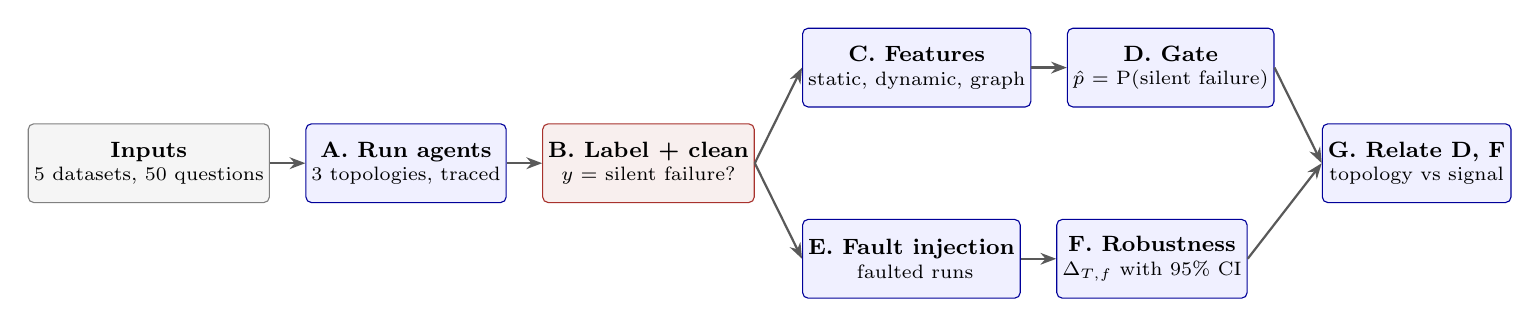
\begin{tikzpicture}[
  node distance=5mm and 4.5mm,
  blk/.style={draw=blue!60!black,fill=blue!6,rounded corners=2pt,minimum width=23mm,minimum height=10mm,inner sep=2pt,
    align=center,font=\footnotesize},
  io/.style={blk,draw=gray,fill=gray!8},
  sf/.style={blk,draw=sfred,fill=sfred!8},
  arr/.style={-{Stealth[length=2mm]},gray!70!black,thick}]
\node[io] (in) {\textbf{Inputs}\\[-1pt]{\scriptsize 5 datasets, 50 questions}};
\node[blk,right=of in] (a) {\textbf{A. Run agents}\\[-1pt]{\scriptsize 3 topologies, traced}};
\node[sf,right=of a] (b) {\textbf{B. Label + clean}\\[-1pt]{\scriptsize $y$ = silent failure?}};
\node[blk,above right=2mm and 6mm of b] (c) {\textbf{C. Features}\\[-1pt]{\scriptsize static, dynamic, graph}};
\node[blk,below right=2mm and 6mm of b] (e) {\textbf{E. Fault injection}\\[-1pt]{\scriptsize \nFaultRuns{} faulted runs}};
\node[blk,right=of c] (d) {\textbf{D. Gate}\\[-1pt]{\scriptsize $\hat{p}$ = P(silent failure)}};
\node[blk,right=of e] (f) {\textbf{F. Robustness}\\[-1pt]{\scriptsize $\Delta_{T,f}$ with 95\% CI}};
\node[blk,below right=2mm and 6mm of d] (g) {\textbf{G. Relate D, F}\\[-1pt]{\scriptsize topology vs signal}};
\draw[arr] (in) -- (a); \draw[arr] (a) -- (b);
\draw[arr] (b.east) -- (c.west); \draw[arr] (b.east) -- (e.west);
\draw[arr] (c) -- (d); \draw[arr] (e) -- (f);
\draw[arr] (d.east) -- (g.west); \draw[arr] (f.east) -- (g.west);
\end{tikzpicture}
\caption{The AgentRel pipeline. Blocks A and B build one labelled corpus; the top branch learns to predict silent
failure, the bottom branch measures robustness under faults, and block G relates them.}\label{fig:pipeline}
\end{figure*}

\section{The AgentRel Framework}\label{sec:framework}
AgentRel sits \emph{outside} the agent. It never changes how the agent reasons; it runs controlled tasks, labels
every run against computed ground truth, learns which signals precede a \SF, and stress-tests the agent's wiring.
Figure~\ref{fig:pipeline} shows the seven blocks; one corpus feeds both branches.

\subsection{Definitions}
A \textbf{run} is one agent topology $T$ answering one phrasing $\pi$ of a question $q$ on dataset $d$ with base
model $M$. Its \textbf{trace} $\tau$ is the ordered list of tool calls (tool, arguments, output, success, retry flag,
latency) plus token counts and the final free-text answer. Let $a$ be the answer parsed from that text and $a^*$
the value a deterministic pandas script computes for $q$. The label is
\begin{equation}
  y(\tau) = \mathbf{1}\left[\, a = \varnothing \;\lor\; |a - a^*| > \varepsilon |a^*| \,\right],
  \quad \varepsilon = 0.01
\end{equation}
(for a categorical answer, $a \neq a^*$ after normalising case and punctuation). A failing run is a \SF{} when
$a \neq \varnothing$ and a \emph{visible failure} otherwise. The gate estimates
\begin{equation}
  \begin{aligned}
  \hat{p}(\tau) &= f\big(\phi_{\text{static}}(d,q),\, \phi_{\text{dynamic}}(\tau),\,
  \phi_{\text{graph}}(G(\tau))\big)\\ &\approx P(y = 1 \mid \tau)
  \end{aligned}
\end{equation}
where $G(\tau) = (V, E)$ is the tool-interaction graph: nodes are tools, edge weights count transitions between
consecutive calls. Topology $T$ is never an input to $f$, because it is the variable the robustness study
manipulates. $f$ minimises the class-weighted log loss
\begin{equation}
  \mathcal{L} = -\frac{1}{N}\sum_i \big[w_1 y_i \log \hat{p}_i + w_0 (1-y_i)\log(1-\hat{p}_i)\big]
\end{equation}
with class weights $w_c = N / (2N_c)$, and robustness of topology $T$ to fault $f$ is the increase in failure rate on the same questions,
\begin{equation}
  \Delta_{T,f} = P(y = 1 \mid T, f) - P(y = 1 \mid T, \text{no fault}).
\end{equation}
The midsem proposal defined a relative accuracy drop; the absolute difference stays defined when baseline accuracy
is low and its bootstrap is better behaved.

\subsection{Algorithms}
\begin{algorithm}[H]
\caption{Build the labelled corpus (blocks A, B)}\label{alg:corpus}
\footnotesize
\begin{algorithmic}[1]
\Require datasets $D$, templates $Q_d$ with truth functions, phrasings $\Pi(q)$, topologies $\mathcal{T}$, model $M$
\Ensure corpus $C = \{(\tau, y)\}$
\For{$d \in D,\ q \in Q_d,\ \pi \in \Pi(q),\ T \in \mathcal{T}$}
  \State $\tau \gets \textsc{Run}(T, M, d, \pi)$ \Comment{fresh session, full trace}
  \State $a \gets \textsc{Parse}(\tau.\text{answer})$
  \State $a^* \gets \textsc{Truth}_q(d)$ \Comment{pandas, never the LLM}
  \State $y \gets$ Eq.~(1); kind $\gets$ silent if $a \neq \varnothing$ else visible
  \State $C \gets C \cup \{(\tau, y, \text{kind})\}$
\EndFor
\State $C \gets \textsc{Clean}(C)$ \Comment{flag timeouts; cap at $Q_3 + 1.5\,$IQR}
\end{algorithmic}
\end{algorithm}

\begin{algorithm}[H]
\caption{Train the silent-failure gate (blocks C, D)}\label{alg:gate-train}
\footnotesize
\begin{algorithmic}[1]
\Require corpus $C$; feature maps $\phi_{\text{static}}, \phi_{\text{dynamic}}, \phi_{\text{graph}}$
\Ensure gate $(f, \theta)$
\State $x_i \gets [\phi_{\text{static}}, \phi_{\text{dynamic}}, \phi_{\text{graph}}]$ \Comment{no topology}
\State split $C$ 70/15/15 by template \Comment{no paraphrase leaks}
\State $f \gets$ LightGBM minimising Eq.~(3) on train
\State $\theta \gets \arg\max_t \mathrm{F2}(y_{\text{val}}, \mathbf{1}[f(x_{\text{val}}) \ge t])$
  \Comment{then frozen}
\State report F2, PR-AUC, Brier, ROC-AUC, MCC, ECE, recall@budget on test
\end{algorithmic}
\end{algorithm}

\begin{algorithm}[H]
\caption{Gate an answer before it is shown (\texttt{scripts/gate.py})}\label{alg:gate}
\footnotesize
\begin{algorithmic}[1]
\Require finished run $\tau$, gate $(f, \theta)$, optional review budget $k$
\State $\hat{p} \gets f(\phi(\tau))$
\If{$\hat{p} \ge \theta$} hold the answer; send the run for review
\Else{} release the answer with $\hat{p}$ as its risk score
\EndIf
\State \textit{batch mode:} review the $\lceil kN \rceil$ runs with the highest $\hat{p}$
\end{algorithmic}
\end{algorithm}

\begin{algorithm}[H]
\caption{Topology robustness, cluster bootstrap (blocks E, F)}\label{alg:robust}
\footnotesize
\begin{algorithmic}[1]
\Require questions $Q$ (canonical phrasing), topologies $\mathcal{T}$, faults $F$, baseline $C$, $B = 1000$
\For{$T \in \mathcal{T},\ f \in F,\ q \in Q$}
  \State $s \gets \text{hash}(\text{run\_id}, f) \bmod 3$ \Comment{seeded step}
  \State $\tau \gets \textsc{Run}(T, M, q)$ with $f$ injected once at step $s$
  \State keep $\tau$ only if the fault fired before the answer
\EndFor
\State $\Delta_{T,f} \gets$ Eq.~(4) on realised runs vs.\ baseline runs of the same questions
\For{$b = 1, \dots, B$}
  \State resample templates with replacement; recompute $\Delta_{T,f}^{(b)}$
\EndFor
\State CI $\gets [q_{2.5}, q_{97.5}]$; significant if $0 \notin$ CI
\end{algorithmic}
\end{algorithm}

\section{The Pipeline, Stage by Stage}
Each stage writes an artifact the next one reads, so every stage can be re-run and inspected on its own. Because a
\SF{} in our own measurement would corrupt every downstream number, each stage carries a guard that turns a would-be
silent error into a loud one (Table~\ref{tab:stages}).

\begin{table*}[t]
\caption{Stages, artifacts and guards.}\label{tab:stages}
\footnotesize
\begin{tabularx}{\textwidth}{@{}P{18mm}P{24mm}LP{30mm}L@{}}
\toprule
Stage & Input & What it does & Output & Guard against a silent error\\
\midrule
Data & public CSVs or seeded generators & materialise 5 datasets; 50 templates $\times$ 5 phrasings with pandas ground
  truth & \texttt{datasets/}\allowbreak\texttt{raw}, question banks & truth errors counted (0); every phrasing of a template shares one
  truth value\\
A. Generate & question banks, config & every phrasing through 3 topologies on one model at temperature 0; fresh
  session per run & \texttt{runs.jsonl} & \texttt{-{}-no-mock} fails loudly if the model is unreachable\\
B. Label & \texttt{runs.jsonl} & parse the answer, score Eq.~(1), paraphrase consistency, flatten and IQR-cap &
  \texttt{labelled.parquet} & parser regression tests; a non-baseline corpus never overwrites its labels\\
C. Features & runs + labels & 9 static, 7 dynamic, 3 graph features per run & feature frame & each block asserts
  it produced exactly the schema's keys\\
D. Classifier & feature frame & class-weighted LightGBM \cite{lightgbm} + 4 baselines incl.\ SMOTE \cite{smote}, in scikit-learn \cite{sklearn}; grouped split; F2 threshold on validation &
  \texttt{classifier\_}\allowbreak\texttt{results.json} & raises if a training fold is single-class\\
E. Faults & question banks & one seeded fault per run at step 0--2 & \texttt{runs\_}\allowbreak\texttt{faults.jsonl} & unrealised
  faults tracked and excluded, not counted as survived\\
F. Robustness & both labelled corpora & $\Delta$ per topology $\times$ fault; 1,000 template resamples &
  \texttt{robustness.csv} & baseline restricted to the faulted questions\\
G. Relate & both corpora, robustness & out-of-fold $\hat{p}$, per-topology PR-AUC, drivers, gate recall on fault
  runs & \texttt{relate\_*.csv} & folds grouped by template; topology only selects rows\\
Gate & labelled corpus & fit $f$ on every run; $\theta$ from out-of-fold F2; hold or release new runs
  (Alg.~\ref{alg:gate}) & \texttt{gate.joblib} & threshold set on out-of-fold scores, never on the model's own
  fit\\
Report & \texttt{results/} & figures and both report editions & this PDF & every number read from results\\
\bottomrule
\end{tabularx}
\end{table*}

\subsection{Corpus and agents}
Five datasets of rising difficulty: Titanic \cite{titanic} (887 rows) and UCI Adult Census \cite{adult} (32,561
rows), downloaded; and three seeded synthetic stand-ins with the traits the proposal called for where no stable
download exists: an NYC-taxi-style table (8,000 rows, outliers and mixed types), a heavy-missingness table (3,000
rows) and an Olist-style schema of three tables that needs joins. Ten templates per dataset cover aggregation,
filtering, group comparison, trend and multi-step questions; each is asked canonically and in four paraphrases,
giving $5 \times 10 \times 5 \times 3 = $ \textbf{\nRuns{} runs}.

The three topologies share one model, one tool registry and one prompt preamble, so only the wiring differs:
\textbf{single ReAct} \cite{react} (one reason-act loop that retries once on a loud error),
\textbf{orchestrator-worker} (planner, worker and an inspector that can demand a redo, after LAMBDA \cite{lambda})
and \textbf{peer tool-graph} (loader, transformer and reducer peers, closest to Data Interpreter \cite{datainterp}).
Agents act through eight sandboxed tools and see a preamble that names columns and types but no quantity, so every
number in an answer must come from a logged tool call. All three run on one local model, qwen3:8b
\cite{qwen3}, served by Ollama.

\subsection{Base model}
\FModelChoice

\begin{table}[!ht]
\caption{Model benchmark: canonical phrasing of every template $\times$ 3 topologies, 150 runs a model, on the 41
templates unaffected by two harness issues (Section~\ref{sec:own}).}\label{tab:bench}
\footnotesize
\begin{tabularx}{\columnwidth}{@{}Lrrrr@{}}
\toprule
Model & Fail & Step cap & No tool & s/run\\
\midrule
\tabBenchmark
\bottomrule
\end{tabularx}
\end{table}

\subsection{Evaluation metrics}
Accuracy is never reported: with a large share of correct runs a model that always says ``fine'' scores well and
catches nothing. Each metric in Table~\ref{tab:metrics} answers one question a user of the gate would ask. Every
interval resamples whole templates, since the runs of one template are near duplicates
\cite{kaufman,cameron}.

\begin{table*}[t]
\caption{Metrics.}\label{tab:metrics}
\footnotesize
\begin{tabularx}{\textwidth}{@{}P{30mm}P{70mm}L@{}}
\toprule
Metric & Definition & Question it answers\\
\midrule
F2 \cite{rijsbergen} & $(1+2^2)\,PR / (2^2 P + R)$ & Recall weighted 4$\times$ precision: a missed silent
  failure costs more than a needless review\\
PR-AUC \cite{saito} & area under precision-recall (average precision) & Ranking quality on the failure class, not
  flattered by easy negatives\\
ROC-AUC & $P(\hat{p}_{\text{failure}} > \hat{p}_{\text{success}})$ & Ranking quality, comparable with other work\\
MCC \cite{chicco} & $\frac{TP\cdot TN - FP\cdot FN}{\sqrt{(TP+FP)(TP+FN)(TN+FP)(TN+FN)}}$ & One number using all
  four confusion cells\\
Balanced accuracy & (recall on failures + recall on successes) / 2 & Is the gate fair to both classes?\\
Brier \cite{brier} & $\frac{1}{N}\sum_i (\hat{p}_i - y_i)^2$ & Overall quality of $\hat{p}$ as a probability\\
ECE \cite{guo} & $\sum_b \frac{n_b}{N}\,|\bar{y}_b - \bar{\hat{p}}_b|$ over 10 bins & Does $\hat{p} = 0.3$ mean a 30\%
  chance?\\
Recall@$k$ & share of failures among the $\lceil kN \rceil$ highest-$\hat{p}$ runs & With time to re-check only
  $k$\% of runs, how many silent failures are caught?\\
$\Delta_{T,f}$ CI \cite{efron,cameron} & percentile interval over 1,000 template resamples & Is a topology's
  degradation distinguishable from noise?\\
\bottomrule
\end{tabularx}
\end{table*}

\section{Results}
\subsection{How common are silent failures?}
Of the \nRuns{} baseline runs, \nFail{} (\failRate) failed: single ReAct \failSingle, orchestrator-worker
\failOrch, peer tool-graph \failPeer. \textbf{\nSilent{} of the \nFail{} failures (\silentShare) were \SFs}: the
agent returned a clean answer and nothing in the run signalled a problem. \FFailureRates

\begin{table}[!ht]
\caption{What a failure looks like (baseline corpus).}\label{tab:outcomes}
\footnotesize
\begin{tabularx}{\columnwidth}{@{}P{27mm}rrL@{}}
\toprule
Outcome & Runs & Share & What the user sees\\
\midrule
\tabOutcomes
\bottomrule
\end{tabularx}
\end{table}

\begin{figure*}[t]
\centering
\includegraphics[width=0.72\textwidth]{failure_by_dataset.png}
\caption{Baseline failure rate by dataset and topology.}\label{fig:dataset}
\end{figure*}

\subsection{Can the trace predict a silent failure? (Q1)}
\begin{table}[!ht]
\caption{Held-out test fold (\testN{} runs from \testGroups{} unseen templates, failure rate \testRate). Threshold
chosen on validation.}\label{tab:clf}
\footnotesize
\begin{tabularx}{\columnwidth}{@{}Lccccc@{}}
\toprule
Model & F2 & PR-AUC & Brier & Prec. & Rec.\\
\midrule
\tabClassifier
\bottomrule
\end{tabularx}
\end{table}

\FClassifier

\begin{table}[!ht]
\caption{Extended evaluation over all \oofN{} runs, out of fold (grouped 5-fold CV by template, failure rate
\oofRate): every run is scored by a model that never saw its template.}\label{tab:ext}
\footnotesize
\begin{tabularx}{\columnwidth}{@{}Lll@{}}
\toprule
Metric & Value & 95\% CI (templates)\\
\midrule
\tabExtended
\bottomrule
\end{tabularx}
\end{table}

\begin{figure}[!ht]
\centering
\includegraphics[width=0.95\columnwidth]{review_budget.png}
\caption{The gate as a review queue: share of silent failures caught when only the highest-scored runs are
re-checked.}\label{fig:budget}
\end{figure}

\begin{figure}[!ht]
\centering
\includegraphics[width=0.8\columnwidth]{calibration.png}
\caption{Calibration of $\hat{p}$ (out of fold).}\label{fig:calib}
\end{figure}

\begin{figure}[!ht]
\centering
\includegraphics[width=\columnwidth]{feature_importance.png}
\caption{What the gate relies on (share of LightGBM gain).}\label{fig:importance}
\end{figure}

\FMetrics

\subsection{Which topology holds up when a component breaks? (Q2)}
\nFaultRuns{} fault-injected runs (canonical phrasing $\times$ 3 topologies $\times$ 3 faults); \realised{} had the
fault fire before the agent answered, and only those count. \emph{Corrupted output} is the fault that manufactures
\SFs: the tool succeeds, the value is quietly wrong, and nothing looks amiss. Table~\ref{tab:robust} and
Figure~\ref{fig:robust} give $\Delta_{T,f}$ for every cell.

\begin{table*}[t]
\caption{Failure-rate increase per topology and fault, Eq.~(4), in percentage points. * the 95\% cluster-bootstrap
CI excludes zero.}\label{tab:robust}
\footnotesize
\centering
\begin{tabular}{@{}llrrrlc@{}}
\toprule
Topology & Fault & Baseline & Faulted & $\Delta$ (pp) & 95\% CI (pp) & \\
\midrule
\tabRobustness
\bottomrule
\end{tabular}
\end{table*}

\begin{figure*}[t]
\centering
\includegraphics[width=0.72\textwidth]{robustness_delta.png}
\caption{$\Delta_{T,f}$ with 95\% cluster-bootstrap intervals; right of zero means the fault made the topology fail
more.}\label{fig:robust}
\end{figure*}

\FRobustness

\subsection{Relating the two (block G)}
\begin{table*}[t]
\caption{One row per topology, most robust first. PR-AUC is out of fold; lift divides it by the failure rate.
Flagged = recall of the baseline-trained gate on realised fault runs.}\label{tab:summary}
\footnotesize
\centering
\begin{tabular}{@{}lrrcrrl@{}}
\toprule
Topology & Mean $\Delta$ (pp) & Failure rate & PR-AUC (lift) & Fault fails flagged & Corrupted flagged
  & Main driver\\
\midrule
\tabSummary
\bottomrule
\end{tabular}
\end{table*}

\begin{figure}[!ht]
\centering
\includegraphics[width=0.9\columnwidth]{pr_curves.png}
\caption{Out-of-fold precision-recall per topology.}\label{fig:pr}
\end{figure}

\begin{figure*}[t]
\centering
\includegraphics[width=0.72\textwidth]{fault_recall.png}
\caption{Share of fault-induced failures the gate flags.}\label{fig:faultrecall}
\end{figure*}

Table~\ref{tab:summary} joins the two halves of the study. \FRelate

\section{Discussion}
\begin{itemize}
\FDiscussion
\end{itemize}

\section{\SFscap{} in Our Own Measurement}\label{sec:own}
Three defects would each have produced wrong numbers with no error, which is to say they were silent failures of
the measurement layer itself. We found them by checking results against expectations, and record them because they
are the project's subject in miniature:
\begin{itemize}
  \item \textbf{The answer parser split long integers.} `32561' parsed as 61 and `2000' as 0, so correct runs were
    labelled failures: a first live slice showed 50\% failure against a true 10\%. Fixed, with a regression test.
  \item \textbf{The schema preamble leaked answers.} It printed row counts and missing rates, the literal answers
    to six templates, which then failed at 23\% against 47\% for the rest. It now names columns and types only.
  \item \textbf{Three questions were unanswerable.} The 1.5$\cdot$IQR templates need quartiles and no tool computed
    one, so every model failed them on every topology. A quantile operation was added.
\end{itemize}
The corpus in this report was generated after all three fixes.

\section{Limitations}
\begin{itemize}
\FLimitations
\end{itemize}

\section{Conclusion}
\FConclusion

\begingroup
\small
\setlength{\itemsep}{0pt}
\begin{thebibliography}{30}
\bibitem{cemri} M. Cemri, M. Z. Pan, S. Yang, et al., ``Why do multi-agent LLM systems fail?'' in \emph{Advances in
  Neural Information Processing Systems (NeurIPS), Datasets and Benchmarks Track}, 2025.
\bibitem{longds} K. Xu, X. Lu, S. Qiao, Z. Ding, H. Xu, L. Liang, and N. Zhang, ``LongDS-Bench: On the failure of
  long-horizon agentic data analysis,'' arXiv:2605.30434, 2026.
\bibitem{earlyeval} Y. Shi, Z. Sun, J. Dong, C. Wan, D. Lo, and X. Gu, ``EarlyEval: Cheaper agent evaluation via
  early outcome prediction,'' arXiv:2609.02783, 2026.
\bibitem{agentrx} Microsoft Research, ``AgentRx: Diagnosing AI agent failures from execution trajectories,'' in
  \emph{Proc. 43rd Int. Conf. on Machine Learning (ICML)}, 2026.
\bibitem{huang} J.-T. Huang, J. Zhou, T. Jin, X. Zhou, Z. Chen, W. Wang, Y. Yuan, M. R. Lyu, and M. Sap, ``On the
  resilience of LLM-based multi-agent collaboration with faulty agents,'' in \emph{Proc. 42nd Int. Conf. on Machine
  Learning (ICML)}, PMLR 267:26202--26226, 2025.
\bibitem{masfire} J. Jia, Z. Deng, Z. Chen, Y. Wang, and Z. Zheng, ``MAS-FIRE: Fault injection and reliability
  evaluation for LLM-based multi-agent systems,'' arXiv:2602.19843, 2026.
\bibitem{farquhar} S. Farquhar, J. Kossen, L. Kuhn, and Y. Gal, ``Detecting hallucinations in large language models
  using semantic entropy,'' \emph{Nature}, vol. 630, no. 8017, pp. 625--630, 2024.
\bibitem{somov} O. Somov and E. Tutubalina, ``Confidence estimation for error detection in text-to-SQL systems,'' in
  \emph{Proc. AAAI Conf. on Artificial Intelligence}, vol. 39, no. 23, pp. 25137--25145, 2025.
\bibitem{datainterp} S. Hong, Y. Lin, B. Liu, et al., ``Data Interpreter: An LLM agent for data science,'' in
  \emph{Findings of the Association for Computational Linguistics: ACL 2025}, pp. 19796--19821, 2025.
\bibitem{lambda} M. Sun, R. Han, B. Jiang, H. Qi, D. Sun, Y. Yuan, and J. Huang, ``LAMBDA: A large model based data
  agent,'' \emph{Journal of the American Statistical Association}, 2025.
\bibitem{infiagent} X. Hu, Z. Zhao, S. Wei, et al., ``InfiAgent-DABench: Evaluating agents on data analysis tasks,''
  in \emph{Proc. 41st Int. Conf. on Machine Learning (ICML)}, PMLR 235:19544--19572, 2024.
\bibitem{dabstep} A. Egg, M. Iglesias Goyanes, F. Kingma, et al., ``DABstep: Data agent benchmark for multi-step
  reasoning,'' arXiv:2506.23719, 2025.
\bibitem{react} S. Yao, J. Zhao, D. Yu, N. Du, I. Shafran, K. Narasimhan, and Y. Cao, ``ReAct: Synergizing reasoning
  and acting in language models,'' in \emph{Int. Conf. on Learning Representations (ICLR)}, 2023.
\bibitem{lightgbm} G. Ke, Q. Meng, T. Finley, T. Wang, W. Chen, W. Ma, Q. Ye, and T.-Y. Liu, ``LightGBM: A highly
  efficient gradient boosting decision tree,'' in \emph{Advances in Neural Information Processing Systems 30}, pp.
  3146--3154, 2017.
\bibitem{smote} N. V. Chawla, K. W. Bowyer, L. O. Hall, and W. P. Kegelmeyer, ``SMOTE: Synthetic minority
  over-sampling technique,'' \emph{Journal of Artificial Intelligence Research}, vol. 16, pp. 321--357, 2002.
\bibitem{saito} T. Saito and M. Rehmsmeier, ``The precision-recall plot is more informative than the ROC plot when
  evaluating binary classifiers on imbalanced datasets,'' \emph{PLoS ONE}, vol. 10, no. 3, e0118432, 2015.
\bibitem{brier} G. W. Brier, ``Verification of forecasts expressed in terms of probability,'' \emph{Monthly Weather
  Review}, vol. 78, no. 1, pp. 1--3, 1950.
\bibitem{guo} C. Guo, G. Pleiss, Y. Sun, and K. Q. Weinberger, ``On calibration of modern neural networks,'' in
  \emph{Proc. 34th Int. Conf. on Machine Learning (ICML)}, PMLR 70:1321--1330, 2017.
\bibitem{chicco} D. Chicco and G. Jurman, ``The advantages of the Matthews correlation coefficient (MCC) over F1
  score and accuracy in binary classification evaluation,'' \emph{BMC Genomics}, vol. 21, no. 6, 2020.
\bibitem{kaufman} S. Kaufman, S. Rosset, C. Perlich, and O. Stitelman, ``Leakage in data mining: Formulation,
  detection, and avoidance,'' \emph{ACM Trans. on Knowledge Discovery from Data}, vol. 6, no. 4, 2012.
\bibitem{efron} B. Efron and R. J. Tibshirani, \emph{An Introduction to the Bootstrap}. Chapman \& Hall/CRC, 1993.
\bibitem{cameron} A. C. Cameron, J. B. Gelbach, and D. L. Miller, ``Bootstrap-based improvements for inference with
  clustered errors,'' \emph{The Review of Economics and Statistics}, vol. 90, no. 3, pp. 414--427, 2008.
\bibitem{rijsbergen} C. J. van Rijsbergen, \emph{Information Retrieval}, 2nd ed. Butterworths, 1979.
\bibitem{qwen3} Qwen Team, ``Qwen3 technical report,'' arXiv:2505.09388, 2025.
\bibitem{adult} B. Becker and R. Kohavi, ``Adult [dataset],'' UCI Machine Learning Repository, 1996,
  doi:10.24432/C5XW20.
\bibitem{sklearn} F. Pedregosa, G. Varoquaux, A. Gramfort, et al., ``Scikit-learn: Machine learning in Python,''
  \emph{Journal of Machine Learning Research}, vol. 12, pp. 2825--2830, 2011.
\bibitem{chatgpt} OpenAI, ``Data analysis with ChatGPT,'' OpenAI Help Center, accessed October 2026.
  \url{https://help.openai.com/en/articles/8437071}
\bibitem{claudefiles} Anthropic, ``Create and edit files with Claude,'' Claude Help Center, accessed October 2026.
  \url{https://support.claude.com/en/articles/12111783}
\bibitem{colab} Google, ``Data Science Agent in Colab,'' Google Developers Blog, March 2025.
\bibitem{titanic} Kaggle, ``Titanic: Machine learning from disaster [dataset].''
  \url{https://kaggle.com/competitions/titanic}
\end{thebibliography}
\endgroup

\end{document}
